\documentclass[11pt,a4paper]{article}
\usepackage{graphicx}
\usepackage[cp1250]{inputenc} 
\usepackage[]{units}
\title{Induction time vs detonation cell size using ZND model. Chapman - Jouguet conditions in methane-air mixtures using SDToolbox.}
\author{Jakub Keciek}
\date{Computational methods in combustion\\
Warsaw University of Technology}

\begin{document}
\maketitle

\clearpage
\tableofcontents
\clearpage
% pierwsza sekcja
\section{Introduction}\label{sec:intro}
First purpose of making this report is to show relation between induction time and detonation cell size. The second purpose of making this project is to present a study of the CJ conditions in various methane - air mixtures. The calculations were made with ZND 
(http://shepherd.caltech.edu/EDL/public/\\
cantera/html/SD$\_$Toolbox/ZND) and SDToolbox ("wang\_highT" mechanism and two functions: "CJSpeed" and "Postshock\_eq").

\section{Mathematical model for ZND}\label{sec:model}
One-dimensional detonation theory proposed by Zeldovich, von Neumann and Doring in 1940s. It tells us the detonation front consists of two phases: compression by shockwave and a finite combustion zone.
Important parameter of a all burning mixtures is detonation cell size. The smaller the value, the more susceptible the mixture is for detonation. A lot of experiments have shown that size of detonation cell is linearly dependent on induction time.

\begin{equation}
    \lambda = a t_i
\end{equation}


Where:\\
$\lambda$ - detonation cell width\\
$a$ - linear coefficient\\
$t_i$ - induction time\\ 


\section{Mathematical model for SDToolbox}\label{sec:model}
Base of solver is simple, 1-dimensional detonation model, proposed by Chapman and Jouguet at turn of XIX and XX century. In that model the detonation wave is a discontinuity in flow.There are applicable three basic conservation laws: mass, momentum and energy.

\begin{equation}
    \rho_1 w_1 = \rho_2 w_2
\end{equation}
\begin{equation}
    p_1 + \rho_1 w_1 u_1 =p_2 + \rho_2 w_2 u_2
\end{equation}
\begin{equation}
    \frac{1}{2} w_1^2 + \frac{\kappa}{\kappa - 1} \frac{p_1}{\rho_1} = \frac{1}{2} w_2^2 + \frac{\kappa}{\kappa - 1} \frac{p_2}{\rho_2} + H
\end{equation}

Where:\\
$p$ - pressure\\
$\rho$ - density\\
$w$ - velocity of shockwave propagation\\
$u$ - velocity of gas\\
$H$ - heat coming from chemical reaction\\
Parameters "1" - in front of shockwave, "2" - parameters behind the shockwave.\\

\section{Results for ZND}\label{sec:results}
Figure 1, shows detonation cell size for some kinds of fuel for varying concentration values. For methane we can see that size of cell is nearly constant, with nearly constant concentration. But looking at figures 1 and 2 we can see a very similar graph shape in other fuels, which confirms the idea, that the relation between these two parameters, induction time and detonation cell size, is indeed linear.\\

\begin{figure}[h]
    \centering
    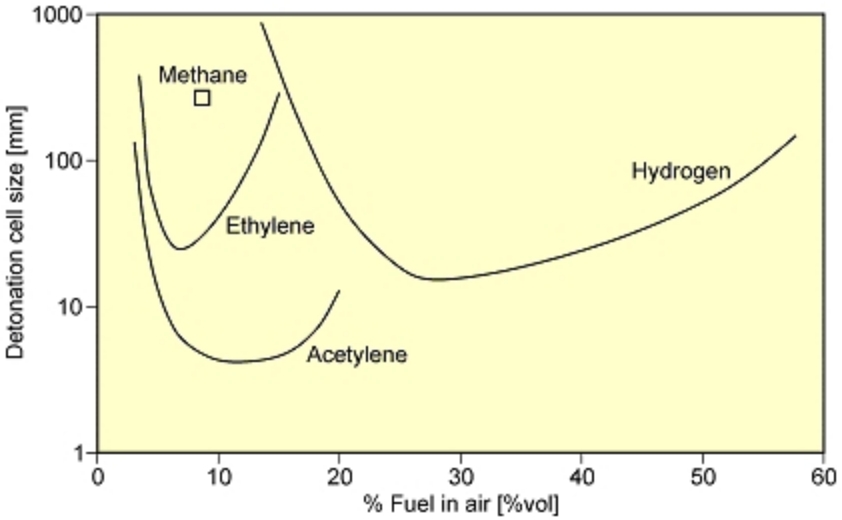
\includegraphics[width=0.6\textwidth]{komorkadetonacji}
    \caption{Detonation cell size for various mixtures}
    \label{fig:A}
\end{figure}

\begin{figure}[h]
    \centering
    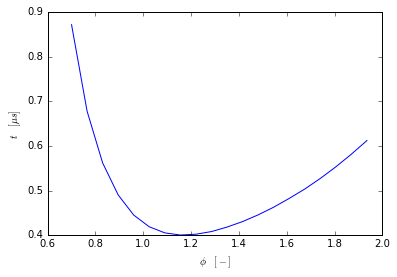
\includegraphics[width=0.6\textwidth]{wykres}
    \caption{Induction time acquired from calculations}
    \label{fig:B}
\end{figure}
Using data obtained from the graphs, we can calculate:\\
\begin{equation}
\lambda = 0.2m, \quad t_i = 0.4 \mu s
\end{equation}

\begin{equation}
	a= \frac{\lambda}{t_i} = 0.5 \left[ \frac{m}{\mu s} \right]
\end{equation}
which is a proportional constant between these two parameters for methane.\\


\section{Results for SDToolbox}\label{sec:results}
There were three series of calculations:\\
Constant temperature T=297K in front of wave (variable pressure and equivalence ratio).\\
Constant pressure P=1bar in front of wave (variable temperature and equivalence ratio).\\
Constant equivalence ratio Phi=1 in front of wave (variable pressure and temperature).\\
The following plots show three basic parameters of a detonative combustion - CJ speed, pressure and temperature behind the wave.\\


Calculations for constant temperature T=297K (variable pressure and equivalence ratio).\\
\begin{figure}[h]
    \centering
    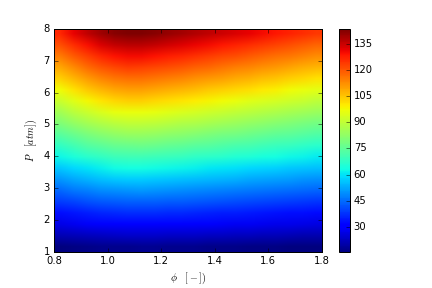
\includegraphics[width=0.7\textwidth]{CJ_P_phi_P_}
    \caption{Chapman Jouguet pressure vs equivalence ratio and pressure}
    \label{fig:C}
\end{figure}
\clearpage
\begin{figure}[t]
    \centering
    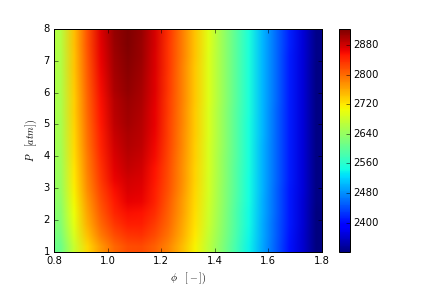
\includegraphics[width=0.8\textwidth]{CJ_T_phi_P_}
    \caption{Chapman Jouguet temperature vs equivalence ratio and pressure}
    \label{fig:D}
\end{figure}

\begin{figure}[b]
    \centering
    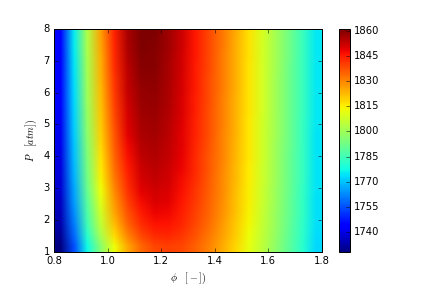
\includegraphics[width=0.8\textwidth]{CJ_V_phi_P_}
    \caption{Chapman Jouguet speed vs equivalence ratio and pressure}
    \label{fig:E}
\end{figure}
\clearpage
Calculations for constant pressure P=1bar(variable temperature and equivalence ratio).\\
\begin{figure}[h]
    \centering
    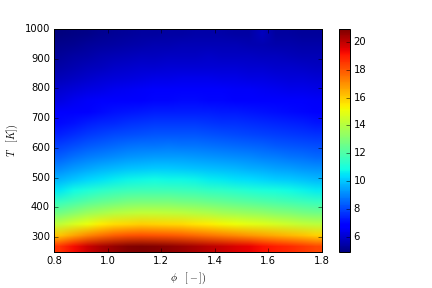
\includegraphics[width=0.7\textwidth]{CJ_P_phi_T_}
    \caption{Chapman Jouguet pressure vs equivalence ratio and temperature}
    \label{fig:F}
\end{figure}

\begin{figure}[h]
    \centering
    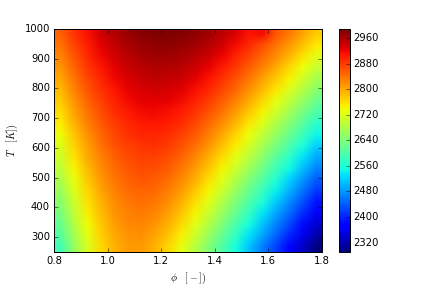
\includegraphics[width=0.7\textwidth]{CJ_T_phi_T_}
    \caption{Chapman Jouguet temperature vs equivalence ratio and temperature}
    \label{fig:G}
\end{figure}
\clearpage
\begin{figure}[h]
    \centering
    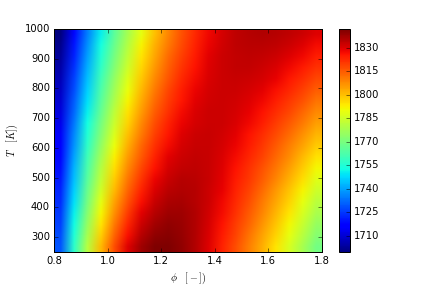
\includegraphics[width=0.7\textwidth]{CJ_V_phi_T_}
    \caption{Chapman Jouguet speed vs equivalence ratio and temperature}
    \label{fig:H}
\end{figure}

Calculations for constant equivalence ratio Phi=1 (variable pressure and temperature).\\
\begin{figure}[h]
    \centering
    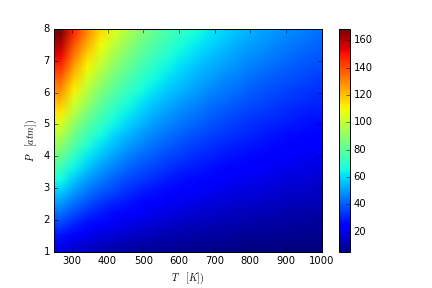
\includegraphics[width=0.7\textwidth]{CJ_P_T_P_}
    \caption{Chapman Jouguet pressure vs temperature and pressure}
    \label{fig:I}
\end{figure}
\clearpage
\begin{figure}[h]
    \centering
    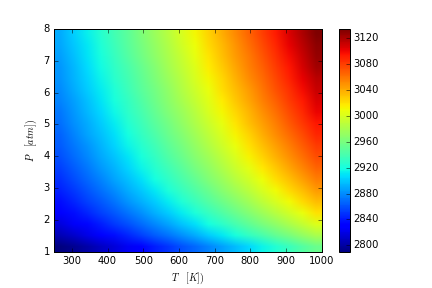
\includegraphics[width=0.7\textwidth]{CJ_T_T_P_}
    \caption{Chapman Jouguet temperature vs temperature and pressure}
    \label{fig:J}
\end{figure}

\begin{figure}[h]
    \centering
    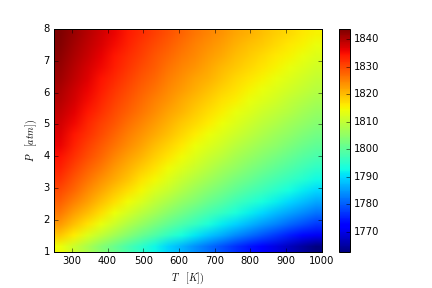
\includegraphics[width=0.7\textwidth]{CJ_V_T_P_}
    \caption{Chapman Jouguet speed vs temperature and pressure}
    \label{fig:K}
\end{figure}

\section{Summary}\label{sec:summary}
- We can experience that induction time is a linear function of detonation cell size.\\
- For constant temperature in front of shockwave pressure is nearly independent of equivalence ratio.\\
- Maximal temperature growth for constant temperature in front of shockwave is for equivalence ratio 1.1.\\
- Maximal speed growth for constant temperature in front of shockwave is for equivalence ratio 1.2.\\
- For constant pressure in front of shockwave pressure is nearly independent of equivalence ratio.\\
- Growth of temperature is increasing to equivalence ratio 1.1 and decreasing from that point for constant pressure in front of shockwave.\\
- Growth of speed is nearly linear for constant pressure in front of shockwave.\\
- For constant equivalence ratio pressure growth is nearly linear.\\
- For constant equivalence ratio temperature is changing asymptotically.\\
- For constant equivalence ratio speed growth is nearly linear.\\

\section{References}\label{sec:refs}

[1] Kordylewski Wlodzimierz, Spalanie i paliwa, Oficyna Wydawnicza Politechniki Wroclawskiej, 2005






\end{document}
